\subsection{Political connections}
\citet{pena2018privatization} use data from 1995-2003 for 25 European countries to conclude that the perceived level of corruption increases with privatizations, however, the impact increase with the economic relevance of the privatization. This could perhaps be a factor in explaining the consistent low level of perceived corruption in Denmark regardless of the evidence of a wide transfer of rent to firms owned by family members to local politicians \citep{amore2013value}. In Spain, a country in which perceived corruption is significantly higher
\citep{amore2013value,pena2018privatization,albalate2017weakening}


\subsection{Political culture in Japan}
Some text
\begin{table}[H]
  \centering
  \footnotesize
  \caption{Corruption Perceptions Index (CPI) 2017.\\
  A score of $0$ is highly corrupt and a score of $100$ is very clean.}
    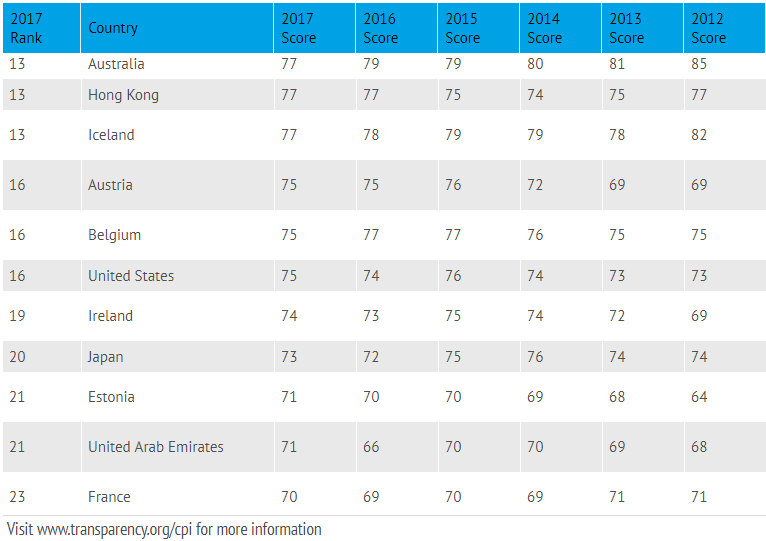
\includegraphics[width= \textwidth]{04_tables/CPI}
  \source{Transparency International.}
  \label{tab:CPI}
\end{table}



 
\subsection{Japanese municipal mergers}
Quite a lot of \href{https://scholar.google.es/scholar?q=japanese+municipal+mergers&hl=da&as_sdt=0&as_vis=1&oi=scholart}{litterature} has been about municipal merger in Japan or taking advantage of it.
